\chapter{PROBLEM}

The basic problem in this thesis is how to found appropriate job descriptions by user's resume. The systems will parse the job descriptions to the job models, and store them in database. When user searches the jobs by their resume in the system, the system will compare the resume to all the job models, and return the job descriptions sorted by their similarity value.

The core idea of our algorithm is calculate similarity between resume model and job model.
We give a formal definition of our problem. All of the notations will be used frequently throughout the thesis.

We use $r$ denote the user's resume model, $R$ has some features $f_i$ like academic degree, their major, their skill set and so on. The symbol $J$ is the set of job models stored in the database, $j_i$ is the $ith$ job model. The similarity function $sim(r, j)$ gives the similarity value between resume $r$ and job $j$. The return list of search function $search(r,J)$ will calculate all the similarity value in the database, and the result of the function will be the job description list ranked their similarity value. The equation of how to calculate similarity value is given below:

$$ sim(r, j) = \sum_{i=1}^{n} simfun_i(r_i,j_i) \times w_i $$

The value of $sim(r, j)$ is summation of similarity value of different fields times their corresponding weight, which means different fields like major and skills,  may have different approaches to calculate their similarity value. We will describe the similarity functions of individual fields in later parts.



\chapter{System Overview}

\section{System Features}
The system will use rule based information extraction technique to parse the job description and resume, and get information such as skill, specialties and background. These information will be used to create the model of job description and job seeker.  Ontology will be used to construct the knowledge base, which will include the taxonomy and rules, to support resume-job matching.

The model of candidates will include their specialties, working experience and education background, all the them should be extracted from the resumes. The job model will be extracted from job description, the information will include: company name, location, job title, education requirement, skill requirements and working experiences etc. When a job seeker searches the jobs by his resume, the system will calculate the similarity between the candidate model and the job models, give every job model a similarity score.

In the initial phase I will only focus on the positions of IT job, because IT jobs have a special character,  skill set oriented, which means the person that the company want to hire must have some special skills and knowledge, like some programming languages, databases or software etc.

User��s personal preference should be considered as well. In the previous user survey, some factors will impact a lot on the user��s expectation of good jobs, such factors include: location, the reputation of the company, the salary etc. These factors will be treated as weight factors in the job matching algorithm.

\section{System Architecture}

Figure ~\ref{fig:Pipeline} shows the architecture of the whole system, which include such modules:

\begin{enumerate}
    \item The web scrawler could search and download all new IT job opening web pages  from indeed.com everyday.
    \item Job parser could parse the job opening web page, extract the information and create the job model.
    \item Resume Parser is much like the Job parser, it will parse the resume and create the candidate model.
    \item All the job models will be stored in the Job Description database.
    \item When user make a query request, the ontology matcher will calculate the matching score of each job, return the jobs ranked by their scores.
\end{enumerate}

\begin{figure}[htbp]
  \centering
  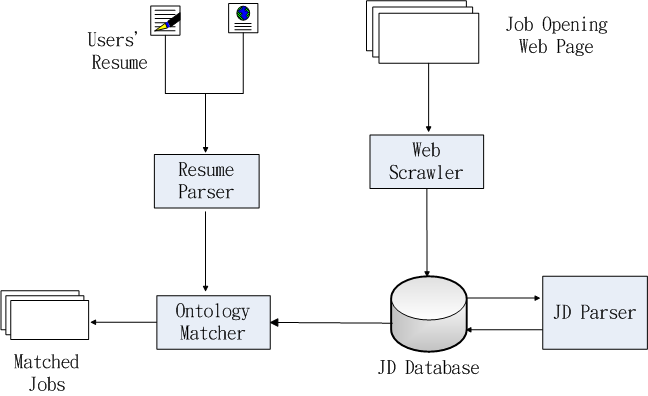
\includegraphics[scale=0.5]{images/arch.png}
  \caption{System Architecture}
  \label{fig:arch}
\end{figure}

\section{System Implementation}

We describe some implementation details here. The whole system was implemented in Python, and used some third party libraries and frameworks. For the web module we used Flask, a lightweight web framework. We used Rdflib as the OWL file parser, PLY(Python Lex-Yacc) as the token regular expression compiler, whoosh as the unversed index builder and Beautiful Soup as the HTML parser.  All the jobs get by the web crawler are stored in the MongoDB NoSQL database.  For the natural language processing part, we used NLTK and pattern to extract the sentences and tokenized the sentences.  

\section{System Interface}

The system provide some interface to end users. The most important interface include review all the jobs in the database, search the jobs by keyword Figure~\ref{fig:joblist},  upload user resume ~\ref{fig:upload_resume}, the resume matching result~\ref{fig:match_resume} and search the jobs with both keyword and resume~\ref{fig:keyword_resume}.

\begin{figure}[htbp]
  \centering
  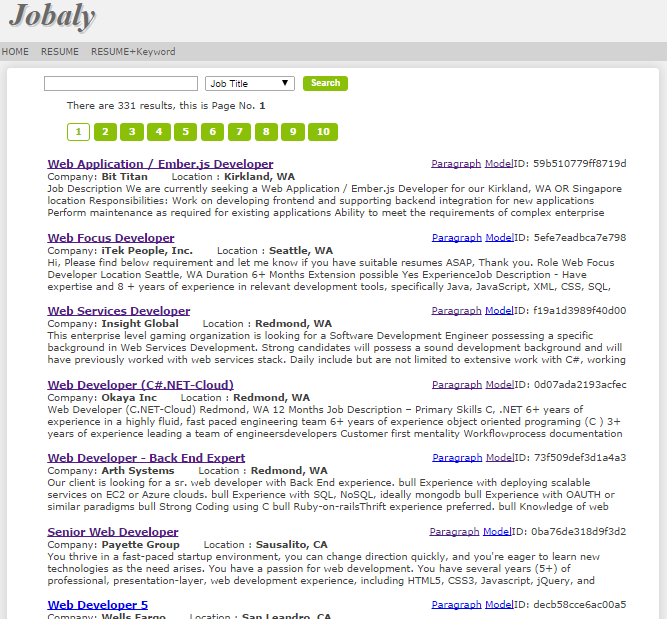
\includegraphics[scale=0.5]{images/joblist.png}
  \caption{System Architecture}
  \label{fig:joblist}
\end{figure}


\begin{figure}[htbp]
  \centering
  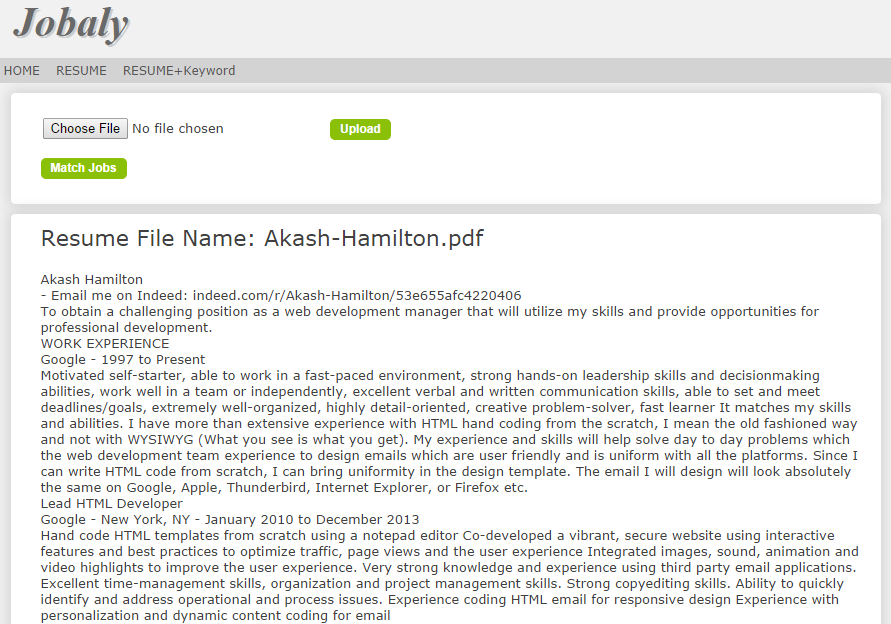
\includegraphics[scale=0.5]{images/upload_resume.png}
  \caption{System Architecture}
  \label{fig:upload_resume}
\end{figure}

\begin{figure}[htbp]
  \centering
  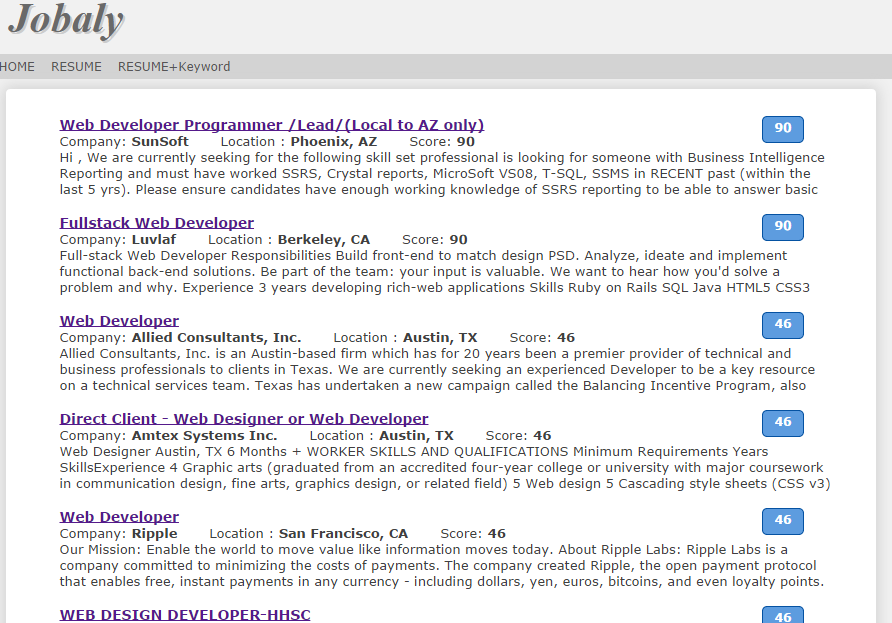
\includegraphics[scale=0.5]{images/match_resume.png}
  \caption{System Architecture}
  \label{fig:match_resume}
\end{figure}

\begin{figure}[htbp]
  \centering
  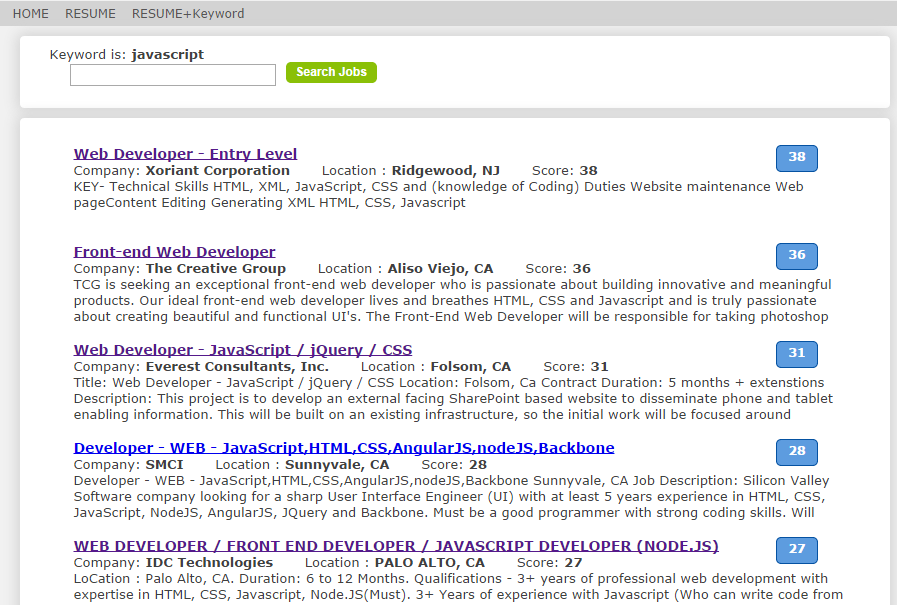
\includegraphics[scale=0.5]{images/keyword_resume.png}
  \caption{System Architecture}
  \label{fig:keyword_resume}
\end{figure}




 

